\documentclass[plain]{sigplanconf}
\usepackage{balance} % For balanced columns on the last page
\usepackage{amsmath}
\usepackage[T1]{fontenc}
\usepackage{lmodern}
\usepackage{graphicx}
\usepackage{amssymb}
\usepackage{tikz}
\usepackage{array}
\usepackage{longtable}
\usepackage[
bookmarksopen,
bookmarksdepth=2,
breaklinks=true
]{hyperref}
\usepackage{natbib}
\setcitestyle{square,sort,comma,numbers}
\makeatletter
\def\BState{\State\hskip-\ALG@thistlm}
\makeatother

\makeatletter
\def\@copyrightspace{\relax}
\makeatother
\begin{document}
	\title{Community Networks QoS Monitoring System}
	\authorinfo{Meluleki Dube}
	{Department of Computer Science\linebreak University of Cape Town\linebreak South Africa}
	{}
	\authorinfo{David Kheri}
	{Department of Computer Science\linebreak University of Cape Town\linebreak South Africa}
	{}
	\authorinfo{Clayton Sibanda}
	{Department of Computer Science\linebreak University of Cape Town\linebreak South Africa}
	{}
	\maketitle
	\begin{abstract}
		
	\end{abstract}
	\begin{CCSXML}
		<ccs2012>
		<concept>
		<concept_id>10003033.10003079.10011704</concept_id>
		<concept_desc>Networks~Network measurement</concept_desc>
		<concept_significance>100</concept_significance>
		</concept>
		</ccs2012>
	\end{CCSXML}
	\ccsdesc[100]{Networks~Network measurement}
	\keywords
	Community Networks, Data-driven Networking, Quality of Services
	
	 \section{Project Description}
This project will build a distributed platform for collecting and analysing Internet quality of service (QoS) metrics within the context of a wireless community network. The platform should be able to help detect sub-optimal or anomalous traffic flows, such as due to misconfiguration or network attacks.
\paragraph{}
This project is three fold: first to help community members understand the performance and utilisation of the network; secondly to help network administrators monitor and detect sub-optimal performance and lastly to help researchers manage and collect data.
\paragraph{}
To achieve this, the project will build a set of distributed Internet measurement units to gather Internet performance datasets in community networks. In addition, the monitoring system will incorporate feature selection mechanisms for detecting and correlating factors impacting network QoS.
\paragraph{}
The final output will be an intelligent QoS system that incorporates network measurements infrastructure and data processing pipeline. As a case study, this project will carried out within the context of iNethi Community Network, a localized content sharing and services platform being developed in Ocean View, a township in Cape Town.


\subsection{Project Significance}
Network measurement tools are now important to all users from administrators to general users. Without measurement platforms that provide a clear visualisation of network activity, administrators must scroll through long unorganized tables of data collected from the network to make sense of the activity in the network. This is an inefficient and time consuming task which deters the detection anomalous behaviour.
\paragraph{}
With a large number of people getting connected, users often want to know their network usage and their footprint on the internet. For example a user maybe interested in knowing the data they consumed over a specific amount of time, the services they use the most or how often they use the internet. Users also want this data delivered in a user friendly way hence the need for an elegant tool to visualise the data.
\paragraph{}
This project therefore aims at building a distributed platform for collecting and analysing internet quality of service(QoS) metrics within the context of a wireless community network. The platform should be able to help detect sub-optimal or anomalous traffic flows, such as due to misconfiguration or network attacks.

\subsection{Issues and Difficulties}
There has been industrial and academic endeavours to characterise the internet through network measurements. However none of the prominent tools have been used in a significant way in developing regions especially in wireless community networks.
\paragraph{}
One of the challenges is that community networks are vastly different from known large common Internet networks. They are implemented using cheap hardware and networking methods. Most of them also have very few physical connections within the network. This gives them a unique architecture which poses a big challenge when it comes to implementing a traditional network measurement tool \cite{Braem:2013:CRC:2500098.2500108}.

Community networks are also plagued with cyber security risks as user privacy may not be guaranteed. Network measurement tools have been suspected to lead to cyber security back doors in networks. 



	\section{Problem Statement}
\subsection{Aims and Research Question}
Community networks are decentralized communication networks which are large scale and self organized, built by the people for the people\cite{Braem:2013:CRC:2500098.2500108}. These networks provide a sustainable solution to address the connectivity gaps that exist in underserved urban, remote, and rural areas around the world\cite{Braem:2015:AEQ:2830629.2830639}. Prominent Examples include Zenzeleni, Rhizomatica and Inethi which is our case study for the project.  

Inethi which is a community network seeks to work with communities to co-design a content sharing and services platform for community wireless networks\cite{inethi}. Its goal is to build more resilient communities by using information technologies to help its users tap into local creativity, innovation, and other resources, with an eye towards improvement of socio-economic status\cite{inethi}.

The aim of this project is to provide researchers and operators of the network with a tool they can use to perform measurements on the community network, also with the ability to schedule collection of network data at specified times. The project also aims to provide end users with the ability to view their data usage accurately in a very user friendly manner. All the functionality discussed previously will be collectively packaged together with a easy to use visual interface. The ultimate goal of the application is to use the data collected enhance quality of service, prevent attack on the network as well as contribute further to the research in community networks.

The main question that we will be seeking to answer with the project are as follows:
\begin{itemize}
	\item How do different measurement collection techniques compare to each other in terms of power efficiency and network efficiency. Where network efficiency focuses on the effects of collecting measurements on the network. Power efficiency looks into the effects on power utilization on of the measurement collection technique used.
	\item How effective are different measurement scheduling mechanisms on data collection 
	\item How efficient different network probing mechanisms are in network analysis 
    \item investigate the effect of co-design process for network based web application interface through usability evaluation
\end{itemize}

\subsection{Requirements}
Our research takes on the form of a software engineering project with members of the Inethi community network as the primary user of the application. The application needs to meet their requirements for it to be of use.
Requirements of the application are as follows 
\begin{itemize}
	\item Provide functionality to perform measurements on the network based on different user-defined fields such latency, signal strength or throughput.
	
	\item Enable the scheduling of network measurements either on demand or at specified time.  
	
	\item Detection of anomalies in the network based on the analysis of the data collected in the network.
	
	\item Creation of user profiles which can be use to track their data usage in the network. 
	
	\item Provide data visualization to both end users in the viewing of their user profiles as well to network operators in the monitoring of the network.
\end{itemize}
Thorough testing and prototyping is paramount, to ensure we meet the requirements, and to provide Inethi with a tool that they are satisfied with.

	\section{Procedure And Methods}
\subsection{Development Procedure}
We need to develop a phone application that will be the means of collecting measurements for the internet metrics. We have decided to build an android application for the phones and tablets as Android is open and requires less resources to get started. According to \cite{statcounter_global_stats}, Android currently has 35\% of the operating systems market. This shows how popular amongst users android is and thus will be a good platform to consider to build the application for first. 
\paragraph{}
The application that we will be building will be extending the MobiPerf application which is built in Java \cite{m-lab}. Since Android Development is also done in Java it also adds to why we will be focusing on developing for android as it is easier to extend an already existing platform compared to creating one form the beginning.

\paragraph{}
For orchestration,once tests are scheduled the server will initiate jobs to online nodes in the network.Network metrics will be measured using the smartphone application explained above and the results will be piped to the database for storage ready for analysis and displayed by the visualizer.    

\subsection{Visualizer}
The visualiser for this project will be implemented as a full stack application comprising of a rich front-end and a well optimised back end. Before building the app, the team will interview potential users from the community network to gather user requirements. The interviews will be done based on a paper prototype done prior to the interviews.

The python web framework Django will be used to build a visualiser web app from the ground up. The framework will be used to implement an HTTP server that will query data from the database. Data will then be exposed in the form of API endpoints to a front end web framework that will display data in the form of graphs.

The advantage of choosing the Django web framework is that it is a simple framework that is easy to use and comes with most backend functionalities already implemented. Django also has a lot of support in the Python community which makes it a reliable option for this project.

For the front end, the web app will leverage the react.js a JavaScript front end web framework to build user-friendly interfaces. React is a component-based library which allows rapid prototyping of web applications. It also managed by Facebook hence making it a reliable and trustworthy tool to use.

For visualisation, the the visualiser employ multiple different graphs. Line graphs will be used to show behaviours of the network over time, this will make it easy to spot anomalies as the graph spikes or dips. Pie charts and scatter plots will also be used to show different categories in the data. For frequency distributions, the visualiser will make use of histograms.

For testing the visualiser, a number of potential users are going to be recruited and asked to use the app in the presence of one of our team members. As a team we will monitor the users as they navigate the web app. Surveys will also be done so as to get the user's perspective on the usability of the app. Issues will be recorded and the app tweaked accordingly to meet the user requirements.

	\section{Ethical And Legal Issues}
For this project, We have identified that the legal and ethical issues to consider are associated with data collection and data storage. Most specifically the issues arising with collecting data from user phones as well as handling the data collected from the users.

\subsection*{Data Collection}
With Data collection we have to worry of a number of things and these are:
\begin{itemize}
	\item What type of data needs to be collected. This may include going to specific users and getting to what data they consider private and would not want to leave their phones. Sensitive data that will need user's permissions will include their particular location that we will need for other measurements we take to make sense. 
	\item Since the system will need to keep track of the different applications that users will use. In attempts to measure which application used most of the data we will have to also consult first with the users to get their permission to do this. Furthermore we want to look into a way of anonymizing data collected. This is so that when stored on the database, data will not be traceable back to the users. This solution will be adopted from the Live-Lab research project who accomplished anonymizing of data by hashing of user names of the users sending the data \cite{Shepard:2011:LMW:1925019.1925023}. We feel we can adopt that and hash the message that we are sending not the user names. The other data that users need to build their profile for network utilization statistics can be stored locally on the phone so that it is only accessible on their devices and no sensitive data leaves the users' phones.
\end{itemize}
\subsection*{Data Storage}
The storage of data has already been hinted above. We need to store data in a way that will make it almost impossible for who ever is viewing the it to be able to track it to a particular user. That is for each data item no one can be able to detect the identity of a user by looking at the data. At the same time we need to know the different devices we are getting the data from so we can be able to keep track of the number of people using the system. We have already stated that this can be achieved by hashing the user name of the different users just before the data is saved on the database. Hashing ensures that we will have unique keys for the data we will be sending online and at the same time we can keep a count of the different keys to know how many people are using the application.

\paragraph{}
We want to ensure that the user's sensitive data will not get to leave the users phone if necessary. 

	\section{Related Works}
MONROE is a platform for running large-scale measurements and experiments in operational Mobile Brodband networks.MONROE handled experiments that range from continuous latency measurements to real time flows.One of MONROE functionalities' is its ability to trigger nodes to run tests on the network
with the purpose of properly assessing network performance.In the implementation of orchestration functionality for this application we intend to replicate their design so as to provide networks operators with a way to schedule network measurements when required %NEED to Cite      
	\section{Anticipated outcome}
\subsection{System}
For the network managers and general users to see past and near-realtime performance of the network, the platform will employ a rich web based dashboard that will display performance measurement graphs for different servers on the network.
\paragraph{}
The interface will make use of different graphs to represent relevant patterns in the data. For frequency distributions, the tool will make use histograms. Line graphs will also be used to show how the network has been performing for a certain amount of time. The visualiser will use blue and white for its user interface colours as these are simple and common colours.
\paragraph{}
The visualizer will be interactive such that users will be able to customise certain parameters like time so as to view specific data they are interested in. Administrators will also be able to generate visual reports of the network.
\paragraph{}
The dashboard will also include an option for users to see a visualisation showing their past network usage which might include type of content being browsed, amount of data used and how often they use a certain service e.g Facebook.

\subsection{Expected Project Impact}
Large networks contain a lot of packets whose data may not be related and this makes it difficult for network managers to spot anomalous behaviours in the network.
\paragraph{}
Our project will include a visualiser that will clearly display data collected from the network traffic. The visualiser will employ graphs that will clearly show the administrator unusual behaviours like a potential cyber attack or a failure in the network.
Using graphs, the visualiser will be able to show the administrators unusual behaviours like a potential cyber attack or a failure in the network.
\paragraph{}
For general users, the visualiser will make them aware of their present and past activity in the network in the form of graphs.
\subsection{Key Success Factors}
Success factors for the data visualizer:
\begin{itemize}
	\item end-users are able to easily and effectively see their data usage in the network.
	\item Network operators/managers can easily visualize activity in the networks. For example number of users in the network or any point of failure. 
\end{itemize}
Success factors for data collection and storage
\begin{itemize}
	\item Accurately collect data from end user's smartphones based on different criteria such as latency, throughput and signal strength.
	\item Data collected is properly stored in a database and can be easily queried for display.
\end{itemize}
Success factors for orchestration tool
\begin{itemize}
	\item Ability to schedule network measurements on demand or at a user defined time.
	\item Allow selection of different network metrics to run measurements on. 
\end{itemize} 



	\section{Project Plan}
\subsection{Risks and Risk Management Strategies}
The risks for the project can be found on Appendix A. The biggest risk for the project will most likey be getting the community involved by using our application as the data that we will be showing depends on them.
\subsection{Timeline}
The project will run from April 2019 till 31 November 2019. The full timeline for the project is shown in Appendix B as a form of the Gantt Chart and a Milestone table.
\subsection{Required Resources}
The resources required are as follows:
\begin{itemize}
	\item IDE for developing this application. For this we are going to use Android Studio \cite{android_developers}.
	\item  We will need a database system that we will use to store the data that we record. For this we have selected a document store database.
	\item We will need a server that will host the database.
	\item A server for the application is also needed.
	\item We will need users for testing the application.
\end{itemize}
\subsection{Deliverables}
The main deliverables for the application will be a QoS Monitoring system. This will comprise of a mobile application that is capable of collection network measurements from the end users and the firewalls. We will also have an Orchestration tool that will be useful to network administrators and researchers for scheduling and triggering network data collections from devices. Finally, we will have a visualizer tool for users to be able to have a visual idea of the network activity. The other deliverables are as follows:
\begin{itemize}
	\item The Literature Review
	\item The Project Proposal
	\item Presentation of the Proposal
	\item Prototypes of the Systems
	\item Project Website
	\item A final Report
\end{itemize}
\subsection{Milestones}
The milestone for the project can be viewed in Appendix B together with the Gantt Chart. Milestones will include the project deliverables.
\subsection{Work Allocation}
The work is divided between the three people involved, Clayton Sibanda, David Kheri and Meluleki Dube. The division is as follows:
\begin{itemize}
	\item Clayton Sibanda is working on the visualizer tool for the application. This will involve coming up with the website where users will be able to visit to see the network activity and their network activity profiles.
	\item David Kheri who is working on the Orchestration tool that will help researchers and network administrators to trigger and schedule data collection from the end users. David will explore using this tool to confirm potential network threats.
	\item  Meluleki Dube is going to be working on creating the application for measuring data and saving the measured data on a database that will be queried by different users for different reasons. This database will be queried by the visualizer that Clayton is working on and by David on when collecting the network results collected from the devices.
\end{itemize}
	%\nocite{*}
	\bibliographystyle{acm}
	\bibliography{references}
	\section*{Appendix}
\begin{figure*}
	\begin{center}
		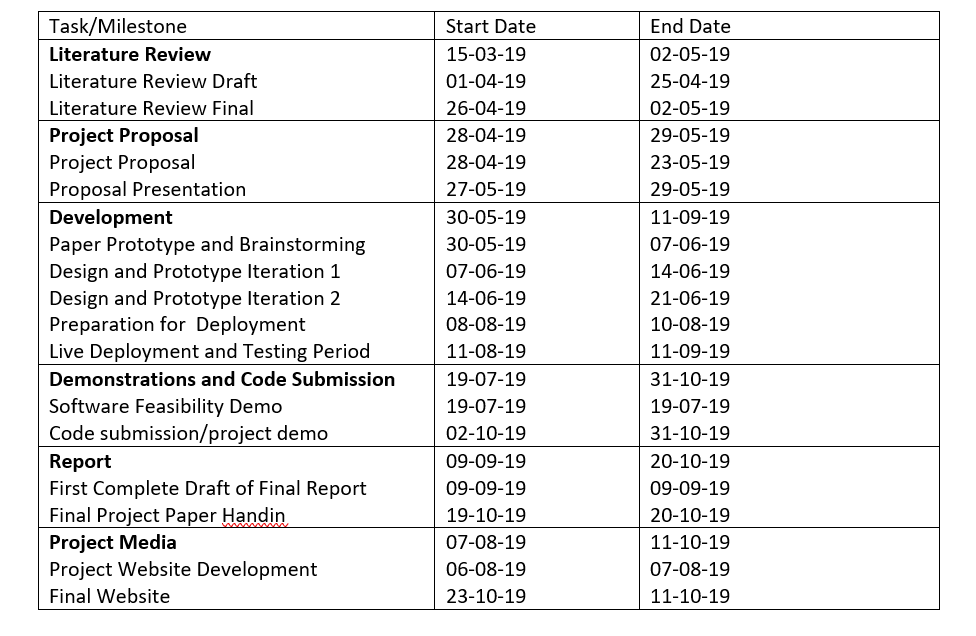
\includegraphics[width=1\linewidth]{res/milestone.png}
	\end{center}
	\caption{Showing time frames at which tasks will be done.}
	\label{fig-ffsm}
\end{figure*}
\begin{figure*}
	\begin{center}
		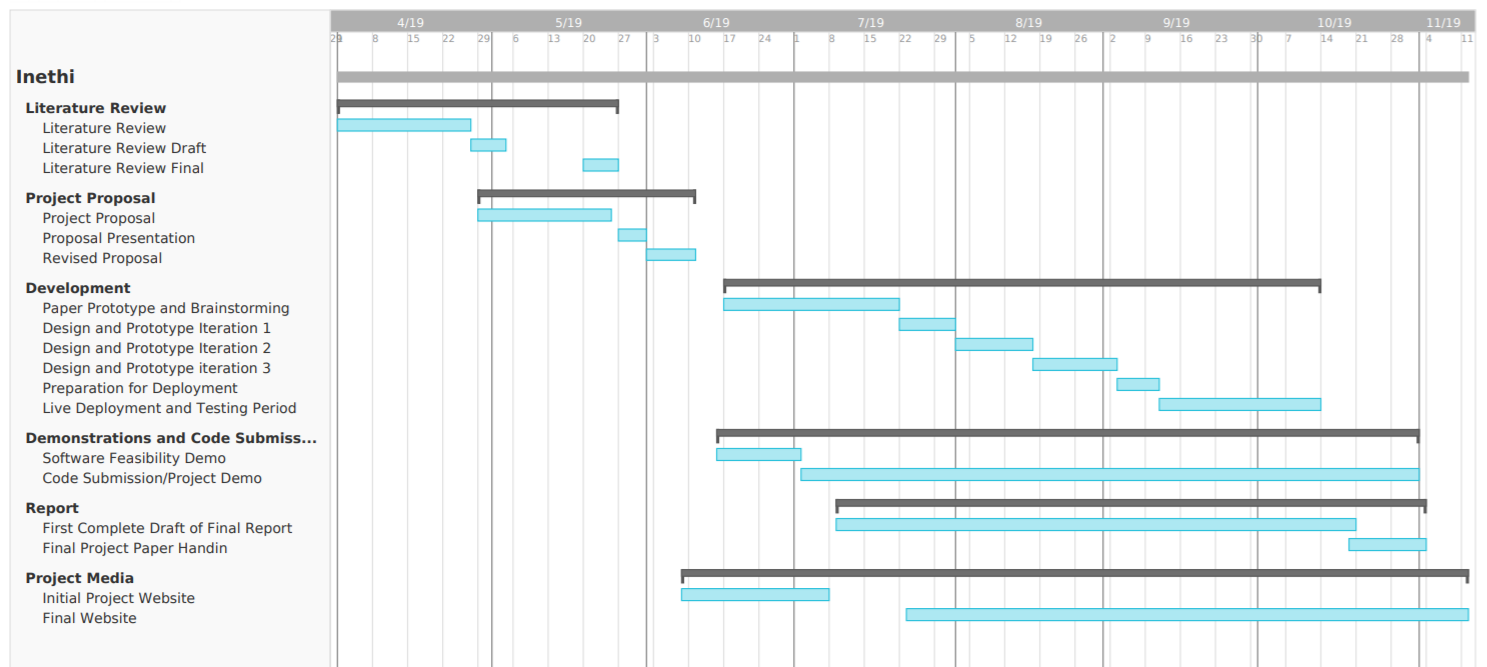
\includegraphics[width=1\linewidth]{res/gantt.png}
	\end{center}
	\caption{Gantt chart showing time frames at which tasks will be done.}
	\label{fig-ffsm}
\end{figure*}
\begin{figure*}
	\begin{center}
		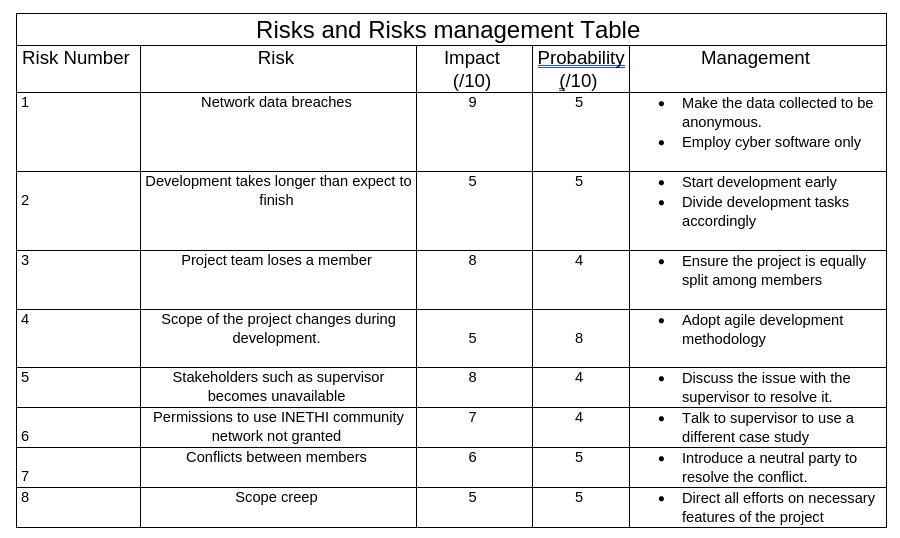
\includegraphics[width=1\linewidth]{res/risks.jpeg}
	\end{center}
	\caption{Showing risks and how they are managed.}
	\label{fig-ffsm}
\end{figure*}
\end{document}